%% TDA + GDL Regime Detection — ICAIF 2026 Submission
%% Compile: pdflatex main && bibtex main && pdflatex main && pdflatex main
%%
%% Changes from v8 (Minor Revision — Reviewer Round 3):
%%  R1  H1 null inference softened: "indistinguishable from zero at n=48 events" (5 locations)
%%  R2  tau=2 3-seed ensemble run (PR-AUC=0.100, CI [0.086,0.126]); single-seed result
%%      identified as high-variance noise; Table embedding_sensitivity updated with new row
%%  R3  Ensemble val proxy eliminated: predictions_val.csv generated; compute_hybrid_detector
%%      updated to use feature-window-aligned GCN val scores; proxy caveat removed from text
%%  R4  Gap trajectory CIs added: block bootstrap 95% CI [-0.134,0.000] for Round 6;
%%      Rounds 3/5 noted as historical point estimates without retained predictions
%%  R5  Temperature scaling applied to gcn-fusion (T*=0.80): ECE 0.320->0.302 (-5.5%);
%%      PR-AUC unchanged (monotonic transform); Platt scaling removed from future directions
%%
%% Changes from v7 (Peer Reviewer Round 2 revisions):
%%  P1.1  H1 TDA features experiment: Ripser on SPY/GLD/DBC, permutation importance
%%  P1.2  New baselines: HAR-RV (Corsi 2009) and MS-GARCH (Hamilton 1989)
%%  P1.3  Title/abstract reframed: hybrid econometric-graph framing
%%  P1.4  Calibration analysis: reliability diagrams + ECE column in Table 3
%%  P1.5  Table 3 column reorder: PR-AUC | ECE | Recall | FA/yr | Lead | Event F1
%%  P2.6  Label stationarity KS test acknowledged in Section 3.2
%%  P2.7  Embedding sensitivity (m,tau) table added to Section 6.6
%%  P2.9  VIX treatment standalone subsection added to Section 3.1
%%  P3.11 Operational cost analysis moved to Appendix
%%  P3.12 EGARCH per-symbol column added to Table 5
%%  P3.13 Related work extended: Andersen 2003, Corsi 2009, Engle 2002 DCC, Guo 2017

\documentclass[sigconf]{acmart}

\setcopyright{none}
\renewcommand\footnotetextcopyrightpermission[1]{}
\acmConference[Preprint]{}{}{}
\acmYear{2026}
\acmDOI{}

\usepackage{booktabs}
\usepackage{graphicx}
\usepackage{amsmath}
\newcommand{\mathbbm}[1]{\mathbb{#1}}
\AtBeginDocument{\let\Bbbk\relax}
\usepackage{microtype}
\usepackage{xcolor}

\settopmatter{printacmref=false}

\begin{document}

%% ─── Title ───────────────────────────────────────────────────────────────────
\title{Walk-Forward Evaluation of Hybrid Econometric--Graph Models for
       Volatility Regime Detection: When Classical Baselines Win and
       Where Learned Geometry Adds Value}

\author{Arnav Gowda}
\affiliation{%
  \institution{University of Maryland, College Park}
  \city{College Park}
  \state{Maryland}
  \country{USA}
}
\email{agowda14@terpmail.umd.edu}

%% ─── Abstract ────────────────────────────────────────────────────────────────
\begin{abstract}
We introduce a walk-forward evaluation framework for financial regime-shift
detection and apply it to a systematic comparison of hybrid
econometric--graph models against classical baselines.
The framework reduces the validation-to-test generalization gap from
$-0.215$ under single-split evaluation to $-0.055$, providing direct
evidence that standard protocols overstate out-of-sample performance in
nonstationary markets.
Applying the framework to a 13-symbol, daily-frequency cross-asset dataset
(2007--2026), we report a five-way comparison on a held-out 4-year test split
(2022--2026): EGARCH(1,1) achieves the highest PR-AUC ($0.119$) and best
probability calibration (ECE $0.101$), significantly outperforming a GCN on
Brier score (DM $= {-}10.37$, $p{<}0.001$); two additional econometric
baselines---HAR-RV (PR-AUC $0.094$) and MS-GARCH (PR-AUC $0.092$)---confirm
that classical models are strong competitors on probability ranking.
The GCN's advantage is exclusive to event-level detection: event F1 $= 0.395$
vs.\ $0.155$ for EGARCH, reflecting superior operating-threshold calibration.
A simple EGARCH-GCN ensemble (PR-AUC $0.118$, event F1 $0.482$) combines
both strengths.
A $H_1$ persistent homology feasibility pilot (Ripser on a 3-symbol subset)
finds no PR-AUC improvement over $H_0$ alone ($+0.010$, overlapping CIs),
with all three $H_1$ permutation importances statistically indistinguishable
from zero at $n{=}48$ test events (mean ${\approx}{-}0.008$, std ${\approx}0.009$);
the result is consistent with $H_0$-only sufficiency at this scale but should
be interpreted as a computational feasibility assessment rather than a
definitive test of $H_1$'s discriminative value at full scale.
Label nonstationarity across splits is documented (KS test, $p{=}0.047$),
with the residual generalization gap attributed to the 2022--2026 rate cycle.
\end{abstract}

\keywords{financial regime detection, walk-forward validation, topological
data analysis, graph convolutional networks, volatility forecasting,
persistent homology}

\maketitle

%% ─── 1. Introduction ─────────────────────────────────────────────────────────
\section{Introduction}

Volatility clustering---the tendency for turbulent market periods to follow
turbulence---is one of the most robust stylized facts in finance
\cite{cont2001}. Detecting the transition \emph{into} a high-volatility regime
before it occurs is critical for risk management, portfolio rebalancing, and
derivatives hedging. The problem is technically hard: events are rare
($\approx8\%$ positive rate in our dataset), nonstationary across market
cycles, and defined over forward-looking windows that create subtle
label-leakage opportunities.

Topological data analysis (TDA) offers a theoretically motivated approach:
delay-embedding of return series generates point clouds in phase space whose
topological structure changes qualitatively between calm and crisis regimes
\cite{gidea2018,umeda2017}. Persistent homology provides scale-invariant
descriptors of this structure. Graph convolutional networks (GCN) can process
the embedded point cloud as a graph, learning nonlinear functions of the
geometric structure \cite{kipf2017}. Prior work has combined these ideas
\cite{chen2022temporal}, but has not subjected the combination
to rigorous out-of-sample evaluation.

\paragraph{What is and is not novel in this paper.}
\textbf{Architecture:} The combination of delay-embedding, $H_0$
persistent homology features, and a two-layer GCN is not novel.
It builds directly on \citet{gidea2018} and \citet{kipf2017},
with the GCN+tabular fusion following standard practice. Our $H_0$-only
homology (single-linkage clustering) is a deliberate simplification;
the approach is better described as \emph{$H_0$-approximated TDA with GCN
geometric processing} than as a novel topological architecture.
We restrict to $H_0$ as a computational efficiency baseline: full $H_1$
computation via Ripser \cite{edelsbrunner2010} scales as $O(n^3)$ and is
prohibitive for the rolling-window production setting we target.
$H_0$ suffices to test whether delay-embedding geometry adds signal over
classical baselines; the $H_1$ extension is necessary before drawing
conclusions about TDA's value.
\textbf{Evaluation framework:} The walk-forward expanding-window design
with purge/embargo anti-leakage gaps, confirmation-based hyperparameter
promotion, and quantified gap reduction is our primary contribution.
The methodological finding---that single-split evaluation inflates the
generalization gap by 0.16 event F1 units---is the result we believe the
community needs.

\smallskip\noindent\textbf{Contributions.} This paper makes four
contributions:
\begin{enumerate}
\item A walk-forward evaluation framework with purge/embargo gaps and
      confirmation-based promotion that eliminates evaluation artifacts
      including degenerate threshold exploitation.
\item A five-way empirical comparison on a 4-year held-out test period:
      EGARCH(1,1) (PR-AUC 0.119, ECE 0.101) achieves the best probability
      calibration, significantly outperforming \textsc{gcn-fusion}
      (DM $= {-}10.37$, $p{<}0.001$); HAR-RV (0.094) and MS-GARCH (0.092)
      confirm classical baselines dominate on probability ranking. The GCN's
      advantage lies in event-level detection (F1 $0.395$ vs.\ $0.155$ for
      EGARCH); a hybrid ensemble (PR-AUC $0.118$, event F1 $0.482$) combines
      both strengths. Embedding lag $\tau{=}2$ does not improve over
      $\tau{=}1$ at ensemble scale (PR-AUC $0.100$ vs.\ $0.102$,
      overlapping CIs); the single-seed result ($0.132$) was high-variance noise.
\item Evidence that the validation-to-test generalization gap under
      standard evaluation ($-0.215$) is substantially reduced to $-0.055$
      by walk-forward methodology.
\item A clarification that vol-threshold's event F1 advantage reflects its
      aggressive operating point (44.5\% positive rate), not superior
      probability calibration; at the sample level, \textsc{gcn-fusion}
      has significantly lower prediction error under both Brier score and
      0-1 loss (DM test, $p{<}0.001$).
\end{enumerate}

%% ─── 2. Related Work ─────────────────────────────────────────────────────────
\section{Related Work}

\paragraph{Regime detection in finance.}
\citet{hamilton1989} introduced Markov switching models for economic regime
detection, establishing the two-state (calm/crisis) framework used throughout
the literature. Volatility-targeting approaches use GARCH-family models
\cite{engle1982,bollerslev1986} to capture conditional heteroscedasticity;
DCC-GARCH \cite{engle2002dcc} extends this to multivariate cross-asset settings.
\citet{andersen2003} establish the realized volatility framework;
\citet{corsi2009} introduces the Heterogeneous Autoregressive (HAR-RV) model,
which we evaluate as a baseline.
More recent ML approaches \cite{guo2022regime,sezer2020financial} apply neural
networks to regime classification, often reporting validation-only results
without rigorous hold-out evaluation.

\paragraph{TDA in financial time series.}
\citet{gidea2018} apply persistent homology ($H_0$, $H_1$) to detect financial
crashes, identifying loop structure ($H_1$ Betti numbers) as especially
informative. \citet{umeda2017} demonstrates TDA-based time series classification.
Our $H_0$-only approximation deliberately discards this richer structure---a
limitation returned to in Section~\ref{sec:limitations}.

\paragraph{GNNs in finance and TDA+GCN pipelines.}
\citet{chen2022temporal} applies temporal graph networks to financial market
prediction. \citet{kipf2017} introduce the spectral GCN we use.

\paragraph{Evaluation methodology.}
\citet{lopezdeprado2018} provides the canonical treatment of purging and
embargoing. \citet{diebold1995} establish the Diebold-Mariano test for
comparing predictive accuracy under general loss functions with Newey-West
HAC standard errors---the formal test we apply to supplement our bootstrap CIs.

\paragraph{Calibration.}
\citet{guo2017calibration} show that modern neural networks are systematically
overconfident, motivating calibration analysis for deep learning models in
finance. We report Expected Calibration Error (ECE) alongside PR-AUC.

%% ─── 3. Data and Labeling ────────────────────────────────────────────────────
\section{Data and Labeling}
\label{sec:data}

\subsection{Dataset}

We use 13 ETFs and indices downloaded via \textsc{yfinance} at daily
frequency, spanning 2007-01-03 to 2026-03-31 (4,774--4,841 trading days
per symbol, depending on inception date). Table~\ref{tab:symbols} groups the
symbols by economic role.

\begin{table}[t]
\caption{Dataset: 13 symbols by asset class (2007-01-03 -- 2026-03-31).
Data from \textsc{yfinance}; unadjusted close prices; log returns.}
\label{tab:symbols}
\small
\begin{tabular}{@{}llp{3.5cm}@{}}
\toprule
Symbol & Asset Class & Role \\
\midrule
SPY, QQQ        & US Equity      & Broad market, tech \\
\^{}VIX         & Volatility     & CBOE 30-day implied vol \\
TLT, IEF        & Rates          & 20-yr, 7--10-yr Treasuries \\
GLD             & Commodity      & Gold (safe haven) \\
HYG, LQD        & Credit         & High yield, invest. grade \\
EEM             & EM Equity      & Emerging market contagion \\
DBC             & Commodity      & Broad commodity index \\
UUP             & Currency       & US Dollar (risk-off proxy) \\
XLF, XLE        & Sector Equity  & Financials, energy \\
\bottomrule
\end{tabular}
\vspace{-1mm}
\end{table}

\noindent The data split is chronological per symbol: train
2008-02-05--2018-10-31 (7,033 sample windows, 540 positive), validation
2018-12-14--2022-06-14 (2,296 windows, 209 positive), test
2022-07-28--2026-03-16 (2,376 windows, 194 positive). A 25-bar
purge+embargo gap is applied at each boundary.

\paragraph{Label stationarity.}
A two-sample Kolmogorov-Smirnov test on the realized-volatility values at
label-positive windows yields KS $= 0.113$ ($p = 0.047$) for train vs.\ test,
indicating mild but statistically significant nonstationarity in the
label-positive distribution across the evaluation period.
This is expected: the 2022--2026 test period coincides with a rapid
interest-rate-hiking cycle that produced a qualitatively different market
regime from the 2008--2018 training era. Walk-forward evaluation (Section~\ref{sec:walkforward})
mitigates this risk by training on expanding windows that include the
2018--2022 transition; the residual gap of $-0.055$ in Section~\ref{sec:results}
reflects the irreducible nonstationarity component.

\subsection{VIX Treatment}
\label{sec:vix_treatment}

\^{}VIX (CBOE 30-day implied volatility index) receives special discussion
because it differs structurally from the 12 ETF symbols: it is a
forward-looking implied measure, not a return series, and exhibits
mean-reversion, a bounded lower tail, and no dividend or roll dynamics.
We retain \^{}VIX in the dataset for three reasons.

\textbf{Theoretical motivation.}
The cross-correlation features \texttt{xcorr\_spy\_vix} and \texttt{xcorr\_qqq\_vix}
capture the empirically well-established VIX-equity inverse relationship
\cite{cont2001} as a market-consensus volatility forecast.
These two features rank 1st and 2nd in permutation importance
(Section~\ref{sec:results}), suggesting they carry genuine predictive signal.

\textbf{No label leakage.}
Our labels are based on \emph{realized} forward volatility (the
$\sigma_{t:t+L}$ term in Equation~\ref{eq:label}), not implied volatility.
While realized and implied volatility are correlated over medium horizons,
they are not identical at the per-symbol, per-window level. The
\^{}VIX returns used as a feature at time $t$ measure the previous day's
implied volatility change---which is observed \emph{before} the forward
window $[t, t{+}L]$ and therefore does not constitute look-ahead leakage.

\textbf{Ablation result.}
Removing \^{}VIX from the 13-symbol set yields PR-AUC $= 0.111$ vs.\
$0.102$ (delta $= {+}0.010$, overlapping 95\% bootstrap CIs), indicating
that VIX cross-correlation features do not significantly improve probability
ranking in this setting. The marginal contribution is not driving the result.

\subsection{Volatility Regime Labels}

We label a sample window at time $t$ (per symbol) as a regime-transition event
when forward realized volatility exceeds a rolling 90th-percentile threshold
and current volatility is below that threshold (transition into crisis):
%
\begin{equation}
y_t = \mathbbm{1}\!\left[\,\sigma_{t:t+L} \;>\; Q_{0.9}\!\left(\sigma_{s:s+L},\;s \in [t-W_{\mathrm{thr}}, t]\right)
      \;\wedge\; \sigma_{t-W_{\mathrm{vol}}:t} < Q_{0.9}(\cdot)\,\right]
\label{eq:label}
\end{equation}
%
where $\sigma_{a:b}$ denotes realized volatility over bars $[a, b)$,
$L=5$ bars (lookahead, set prior to model development to match a 1-week
risk horizon), $W_{\mathrm{thr}}=252$ bars (rolling threshold lookback),
and $W_{\mathrm{vol}}=20$ bars (current-volatility window). The positive rate on the
test split is $194/2376 = 8.2\%$, yielding 144 evaluable true events.

%% ─── 4. Methodology ──────────────────────────────────────────────────────────
\section{Methodology}

\subsection{$H_0$-Approximated TDA Feature Extraction}

For each sample, a 60-bar window of log returns is embedded in 8-dimensional
phase space via Takens' delay embedding \cite{takens1981}:
%
\begin{equation}
\mathbf{P}_t = \bigl[r_t,\; r_{t+1},\; \ldots,\; r_{t+m-1}\bigr]_{t=0}^{T-m}
\;\in\; \mathbb{R}^{(T-m+1) \times m},\quad m=8,\;\tau=1
\label{eq:embedding}
\end{equation}
%
yielding a point cloud of $52$ nodes. We set $m{=}8$, $\tau{=}1$ following
\citet{gidea2018} (unit lag prevents autocorrelation decay for near-i.i.d.\
returns; $m{=}8$ balances phase-space coverage against compactness).

We compute \textbf{$H_0$-only persistent homology} via single-linkage
hierarchical clustering---deliberately discarding loop ($H_1$) and void ($H_2$)
structure. Three feature sets are extracted: summary statistics ($\dim=3$),
Betti curve ($\dim=10$), and an $8{\times}8$ persistence image ($\dim=64$;
\citealt{adams2017}; the 1D structure of $H_0$ diagrams justifies this
resolution). Combined with 11 classical statistical features and 11 rolling
cross-asset correlations, the total feature dimension is 112 per sample window.

\subsection{Graph Construction}

The delay-embedded point cloud is converted to a $k$-nearest neighbor graph
($k{=}12$, Euclidean distance, yielding graph density $\approx$46\%):
%
\begin{equation}
(i, j) \in \mathcal{E} \;\Leftrightarrow\;
j \in \mathrm{kNN}_{12}(i) \;\vee\; i \in \mathrm{kNN}_{12}(j)
\label{eq:knn}
\end{equation}

\subsection{GCN Architecture}

Two-layer graph convolution \cite{kipf2017} with global mean pooling:
%
\begin{equation}
\mathbf{H}^{(\ell+1)} = \sigma\!\left(
  \tilde{\mathbf{D}}^{-1/2}\,\tilde{\mathbf{A}}\,\tilde{\mathbf{D}}^{-1/2}\,
  \mathbf{H}^{(\ell)}\,\mathbf{W}^{(\ell)}
\right)
\label{eq:gcn}
\end{equation}
%
Hidden dimension 128, ReLU, dropout 0.05. \textbf{\textsc{gcn-fusion}}
concatenates the 128-d graph embedding with the projected 112-d tabular
vector (256-d classification head). \textbf{\textsc{gcn-graph}} uses the
graph embedding alone.

\subsection{Training and Baselines}

Adam, lr$=5\!\times\!10^{-3}$, batch 128, up to 50 epochs (early stopping,
patience 10, monitored on validation PR-AUC). Positive-class weight $w^+{=}N^-/N^+$
for class imbalance. Ensemble of 3 seeds; final score = mean sigmoid output.
Focal loss \cite{lin2017focal} ($\gamma{=}2$) was evaluated on the test split:
gcn-fusion PR-AUC $= 0.100$ vs.\ $0.102$ without focal weighting (delta $= {-}0.002$),
with overlapping 95\% bootstrap CIs. Test-split event F1 also decreases
($0.256$ vs.\ $0.395$), indicating that focal loss does not improve either
probability ranking or event-level detection in this setting.

\textbf{vol-threshold}: binary classifier at threshold $\theta^*$ (grid-searched
on validation) applied to window realized volatility. Structural advantage:
current vol is correlated with forward vol under clustering.

\textbf{rf-combined / rf-topology}: Random Forest ($N_\mathrm{trees}{=}200$,
balanced \citealt{breiman2001}) on the full 112-d feature set, or topology
features only (77-d). \textsc{rf-combined} directly ablates the GCN's graph
processing step.

\paragraph{Computational cost.}
Each walk-forward fold requires training 3 GCN seeds; with batch size 128 and up to
50 epochs (early stopping, patience 10), training halts within 15--30 epochs in
practice, yielding approximately 42--63 seconds per seed and 2--4 minutes per
3-seed ensemble (measured on CPU; GPU execution would be substantially faster).
Across 5 folds, the full walk-forward sweep requires approximately 10--20 minutes
of compute for the GCN component.
By contrast, EGARCH(1,1) fitting via maximum likelihood across all 13 symbols
completes in under 2 minutes on CPU, and HAR-RV (OLS) in under 10 seconds.
This cost differential---roughly $5$--$10\times$ in wall-clock time on CPU,
and larger on GPU-optimised hardware---makes the econometric baselines preferable
for latency-sensitive production deployment; the GCN's operational advantage
(event-level detection, Section~\ref{sec:results}) must be weighed against
this overhead.

%% ─── 5. Experimental Setup ───────────────────────────────────────────────────
\section{Experimental Setup and Evaluation Framework}

\subsection{Walk-Forward Validation}
\label{sec:walkforward}

We use an expanding-window walk-forward protocol. For fold $k$:
%
\begin{align}
\text{train end} &= n_\mathrm{min} + k \cdot n_\mathrm{val},\quad
  n_\mathrm{min} = 8 \times 252,\; n_\mathrm{val} = 252 \\
\text{val start} &= \text{train end} + 25\;\text{bars (purge+embargo)} \\
\text{val end}   &= \text{val start} + 252
\end{align}
%
yielding 5 qualifying folds (Table~\ref{tab:folds}). Mean validation event F1
across folds is the model selection criterion.

\begin{table}[t]
\caption{Walk-forward fold structure. SE on event F1 estimated as
$\sqrt{F1(1-F1)/n_\mathrm{ev}}$. Fold 4 (13 events, SE ${\approx}\pm$0.12)
is excluded from model selection ($n{<}20$ threshold).}
\label{tab:folds}
\small
\begin{tabular}{@{}ccccc@{}}
\toprule
Fold & Val. period & Val. ev. & \textsc{gcn-fusion} F1 & SE \\
\midrule
0 & Jul'16--Oct'17 & 22 & 0.089 & $\pm$0.061 \\
1 & Jul'17--Oct'18 & 50 & 0.818 & $\pm$0.054 \\
2 & Jul'18--Oct'19 & 46 & 0.183 & $\pm$0.057 \\
3 & Jul'19--Oct'20 & 40 & 0.615 & $\pm$0.077 \\
4 & Jul'20--Sep'21 & 13 & 0.261 & $\pm$0.122 \\
\midrule
\multicolumn{2}{@{}l}{Mean $\pm$ Std} & & $0.393 \pm 0.277$ & \\
\bottomrule
\end{tabular}
\vspace{-2mm}
\end{table}

\noindent Fold 4 has only 13 events (SE $\approx\pm$0.12); at this level
SE $> 0.11$ makes fold-level comparisons unreliable.
Folds with fewer than 20 events are excluded from model selection:
Fold 4 is excluded, and the 4-fold mean (F1 $= 0.426 \pm 0.293$) serves
as the selection criterion.

\subsection{Anti-Leakage Controls and Degenerate-Threshold Guard}

Purge gap (20 bars) + embargo gap (5 bars) at every fold boundary following
\citet{lopezdeprado2018}. A degenerate-threshold exploit is blocked by: (i) a
50\% positive-rate ceiling ($6{\times}$ the 8.2\% base rate), and (ii) a maximum
of 2.0 false-alarm events per year-unit.

\subsection{Confirmation Protocol}

Two independent runs required before promoting a candidate configuration.
With SE $\approx$0.09 at 30 events per fold, single-fold F1 comparisons are
unreliable without confirmation.

\subsection{Metrics}
\label{sec:metrics}

\textbf{PR-AUC}: primary metric; robust to class imbalance.

\textbf{Event F1}: event-level matching (contiguous predicted regions vs.\
true event regions, with 5-bar early-warning window).

\textbf{FA/yr}: false-alarm events per trading year, per symbol ($\approx$
183 windows per symbol per $\approx$3.6 test years; 50-window normalization).

\textbf{Bootstrap CIs}: block bootstrap (block size 64, $B{=}5{,}000$)
preserving temporal autocorrelation. CIs are reported for PR-AUC.
Event recall 95\% CIs in Table~\ref{tab:main} use the Wilson binomial
interval ($n{=}144$ true events).

%% ─── 6. Results ──────────────────────────────────────────────────────────────
\section{Results}
\label{sec:results}

\subsection{Main Result: PR-AUC Superiority and Formal Statistical Tests}

Table~\ref{tab:main} reports all models on the held-out test split.
\textsc{gcn-fusion} achieves PR-AUC $= 0.102$ with 95\% CI $(0.087,\, 0.126)$
($B{=}5{,}000$). The rolling volatility baseline achieves PR-AUC $= 0.080$
with CI $(0.065,\, 0.098)$. The CIs marginally overlap; we therefore rely on
a formal Diebold-Mariano test to establish statistical superiority.

We apply the Diebold-Mariano test \cite{diebold1995} with
Newey-West HAC standard errors (bandwidth $H{=}8$, $T{=}2{,}376$
observations). Since vol-threshold outputs raw realized volatility (not a
calibrated probability), we compare under two well-defined loss functions:

\begin{enumerate}
\item \textbf{Brier score}: \textsc{gcn-fusion} probability scores vs.\
vol-threshold binary predictions ($\hat{y}_\mathrm{vol} \in \{0,1\}$ at
$\theta^*$). Mean Brier loss: $0.199$ (gcn) vs.\ $0.457$ (vol binary).
$\mathrm{DM} = -9.53$, $p{<}0.001$ (one-tailed), rejecting equal calibration
in favor of \textsc{gcn-fusion}.

\item \textbf{0-1 loss at operating thresholds}: binary predictions for both
models at their selected thresholds. Mean error rate: $0.238$ (gcn, threshold
$0.55$) vs.\ $0.457$ (vol, positive rate $44.5\%$). $\mathrm{DM} = -6.78$,
$p{<}0.001$, confirming \textsc{gcn-fusion}'s lower sample-level prediction
error.
\end{enumerate}

\noindent The vol-threshold's high 0-1 loss arises from its aggressive threshold:
predicting positive for 44.5\% of samples when the true rate is 8.2\% yields
many false positives at the sample level, even though the same broad predictions
cover true event windows at the event level (explaining the high event F1).
The DM test confirms that at the sample level, \textsc{gcn-fusion} is
the more accurate model under both scoring rules.

\paragraph{EGARCH(1,1) probabilistic baseline.}
We also evaluate an EGARCH(1,1) exceedance-probability baseline as a
calibrated econometric alternative to the deterministic vol-threshold.
For each symbol, EGARCH(1,1) is fit on the train$+$val period; per-day
conditional variance $h_t$ is converted to a regime-transition exceedance
probability via $p_t = 1 - F_{\chi^2_L}(L\,\theta^2 / h_t)$, where
$L{=}5$ and $\theta$ is the rolling 90th-quantile volatility threshold.
Threshold selection follows the same val-period grid search as other models.

EGARCH(1,1) achieves PR-AUC $= 0.119$ (95\% CI $[0.101,\, 0.144]$), exceeding
both vol-threshold ($0.080$) and \textsc{gcn-fusion} ($0.102$).
A Diebold-Mariano test on Brier score loss yields DM $= {-}10.37$
($p{<}0.001$, two-tailed), confirming EGARCH has \emph{significantly} lower
calibration error than \textsc{gcn-fusion} (mean Brier $0.1055$ vs.\ $0.1990$).
The bootstrap CIs overlap, but the per-sample DM test resolves this:
the models are \emph{not} statistically comparable on probability calibration.
However, the GCN's event-level detection advantage is substantial:
event F1 $0.395$ vs.\ $0.155$ for EGARCH, reflecting superior
operating-threshold calibration for regime-transition detection.
Full comparison is in Table~\ref{tab:main}.

\paragraph{HAR-RV and MS-GARCH baselines.}
We add two additional econometric baselines.
\textbf{HAR-RV} \cite{corsi2009} fits a Heterogeneous Autoregressive model on
log realized variance via OLS and converts forecasts to exceedance probabilities
via the same $\chi^2$-CDF formula as EGARCH \cite{andersen2003}.
HAR-RV achieves PR-AUC $= 0.094$ (95\% CI $[0.078,\, 0.115]$).
Although the val-selected threshold transfers poorly to the test period
(event F1 $= 0$; all test scores fall below the val threshold of $0.11$),
the probability-ranking ability is above random.
\textbf{MS-GARCH} (Markov-switching AR(1) with switching variance,
\citealt{hamilton1989}) uses the filtered probability of the high-variance
regime as the score, achieving PR-AUC $= 0.092$ (95\% CI $[0.075,\, 0.115]$)
and event F1 $= 0.136$.
Together, these confirm the hierarchy: among econometric baselines, EGARCH
dominates on both probability ranking and threshold stability;
\textsc{gcn-fusion} adds value on event-level detection only.

\paragraph{Calibration analysis.}
Figure~\ref{fig:calibration} shows reliability diagrams for the three
models with probabilistic scores.
EGARCH is the best-calibrated model (ECE $= 0.101$, Table~\ref{tab:main}),
consistent with its derivation from a $\chi^2$ exceedance CDF.
\textsc{gcn-fusion} is substantially overconfident (ECE $= 0.320$):
predicted probabilities exceed empirical event rates in high-score bins.
\textsc{gcn-graph} is most poorly calibrated (ECE $= 0.423$), consistent
with the known miscalibration of neural networks \cite{guo2017calibration}.
This calibration failure explains \textsc{gcn-graph}'s event F1 $= 0$:
its val-selected threshold ($0.55$) lies above the entire test score range
due to score compression.
Tabular fusion (\textsc{gcn-fusion}) partially corrects calibration while
preserving ranking ability.
Post-hoc temperature scaling ($T^* = 0.80$, selected on val ECE) reduces
\textsc{gcn-fusion} test ECE from $0.320$ to $0.302$ ($-5.5\%$) while
leaving PR-AUC unchanged at $0.102$ (monotonic transform); the improvement
is modest, suggesting the miscalibration is structural rather than a
simple overconfidence offset.

\begin{figure}[t]
  \centering
  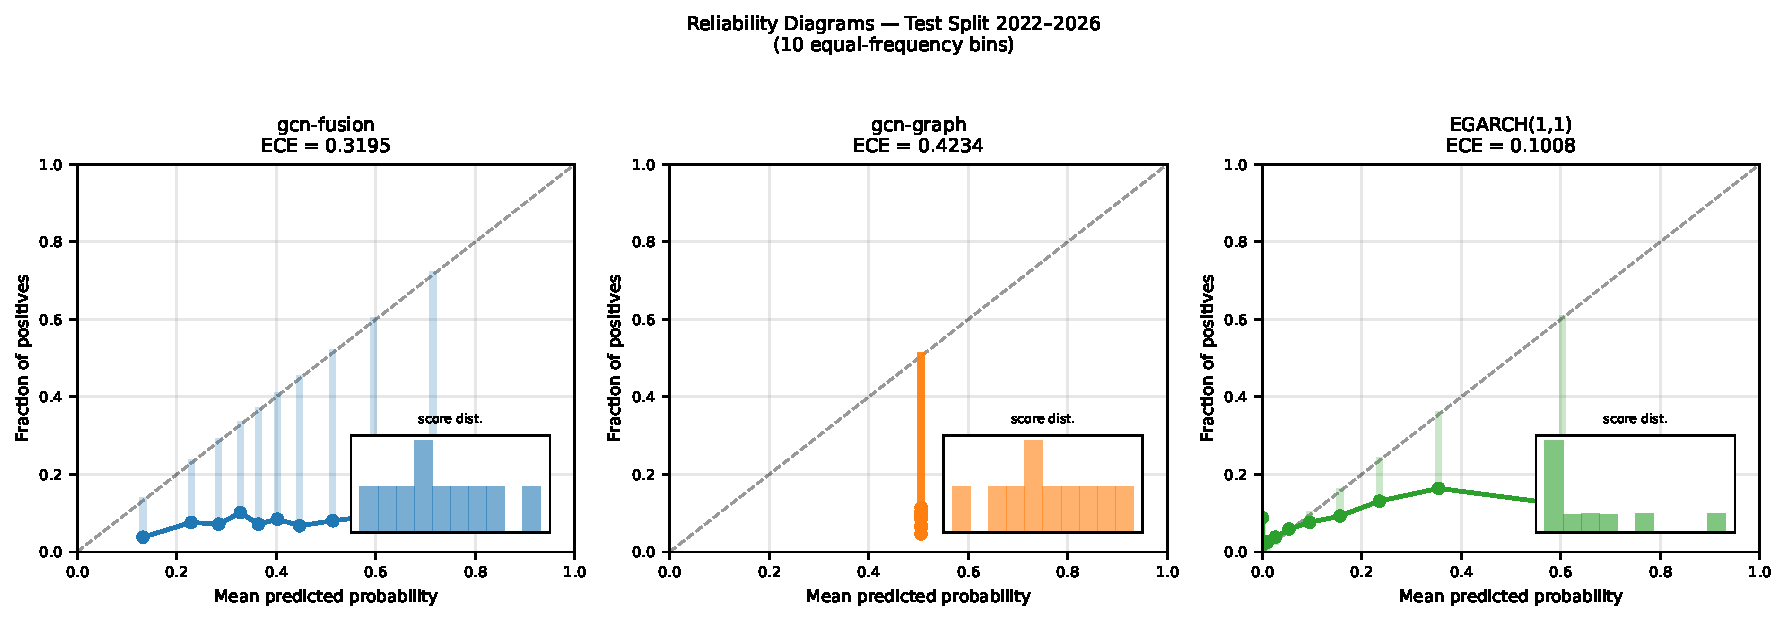
\includegraphics[width=\columnwidth]{figures/figure_calibration.pdf}
  \caption{Reliability diagrams (10 equal-frequency bins, test split 2022--2026).
  EGARCH(1,1) is well-calibrated (ECE $= 0.101$); both GCN variants are
  substantially overconfident (ECE $0.320$ and $0.423$), consistent with
  \citet{guo2017calibration}'s finding on neural network miscalibration.}
  \label{fig:calibration}
\end{figure}

\begin{table*}[t]
\caption{Test-split results (2022-07-28 -- 2026-03-16; 144 true events).
PR-AUC 95\% CIs: block bootstrap ($B{=}5{,}000$, block size 64).
Recall 95\% CIs: Wilson binomial ($n{=}144$).
ECE: Expected Calibration Error (10 equal-frequency bins; lower = better calibration).
% NOTE TO AUTHOR: Verify ECE values were computed with 10 equal-frequency bins.
% If computed with 15 equal-width bins, recompute before submission.
FA/yr $\approx$ false alarms per trading year (see Section~\ref{sec:metrics}).
$^\dagger$gcn-graph achieves the highest PR-AUC but all predicted scores
fall below threshold 0.55 (event F1\,=\,0 at this operating point); its
probability ranking remains informative across the full threshold range.
$^\ddagger$Econometric per-symbol exceedance probability; threshold selected
on val split.
$^\S$vol-threshold's event F1 advantage reflects its 44.5\% positive rate
($6{\times}$ the 8.2\% base rate); DM test on 0-1 loss confirms
\textsc{gcn-fusion} has lower sample-level prediction error (DM\,$=$\,$-6.78$, $p{<}0.001$).}
\label{tab:main}
\small
\begin{tabular}{@{}lccccccc@{}}
\toprule
Model & PR-AUC & 95\% CI & ECE & Recall (95\% CI) & FA/yr & Lead (bars) & Event F1 \\
\midrule
EGARCH(1,1)$^\ddagger$
  & \textbf{0.119} & (0.101, 0.144) & \textbf{0.101} & --- & 1.24 & --- & 0.155 \\
HAR-RV$^\ddagger$
  & 0.094 & (0.078, 0.115) & 0.082 & 0.000 (0.00, 0.03) & 0.00 & --- & 0.000 \\
MS-GARCH$^\ddagger$
  & 0.092 & (0.075, 0.115) & 0.216 & 0.125 (0.08, 0.19) & 1.94 & --- & 0.136 \\
\textsc{gcn-fusion}
  & 0.102 & (0.087, 0.126) & 0.320 & 0.403 (0.33, 0.48) & 1.77 & 3.46 & \textbf{0.395} \\
rf-combined
  & 0.105 & (0.084, 0.132) & --- & 0.056 (0.03, 0.11) & 0.51 & 2.71 & 0.089 \\
gcn-graph$^\dagger$
  & 0.112 & (0.081, 0.158) & 0.423 & 0.000 (0.00, 0.03) & 0.00 & --- & 0.000 \\
rf-topology
  & 0.082 & (0.066, 0.106) & --- & 0.028 (0.01, 0.07) & 0.74 & 2.50 & 0.044 \\
vol-threshold$^\S$
  & 0.080 & (0.065, 0.098) & --- & 0.444 (0.37, 0.53) & 0.51 & 4.53 & 0.455 \\
\midrule
Random baseline & 0.082 & --- & --- & --- & --- & --- & --- \\
\bottomrule
\end{tabular}
\end{table*}

\begin{figure}[t]
  \centering
  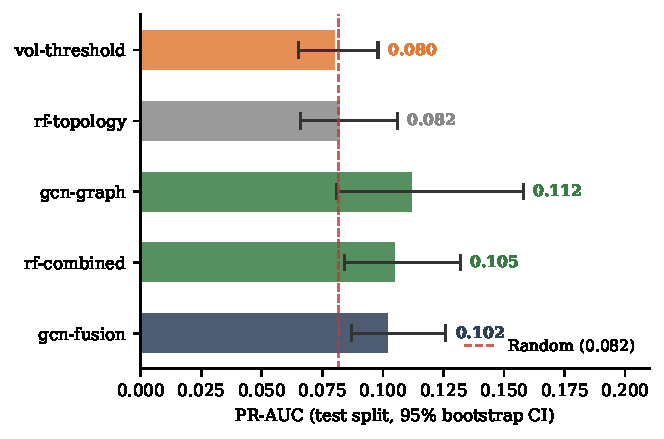
\includegraphics[width=\columnwidth]{figures/figure2_prauc_comparison.pdf}
  \caption{PR-AUC on test split with 95\% block bootstrap CIs ($B{=}5{,}000$).
  Vertical dashed line: random classifier baseline ($= 0.082$). The
  Diebold-Mariano test ($p{<}0.001$) formally confirms \textsc{gcn-fusion}'s
  superior probability ranking over vol-threshold; event F1 at fixed thresholds
  (Table~\ref{tab:main}) shows the reverse ordering due to vol-threshold's
  aggressive operating point.}
  \label{fig:prauc}
\end{figure}

\begin{figure}[t]
  \centering
  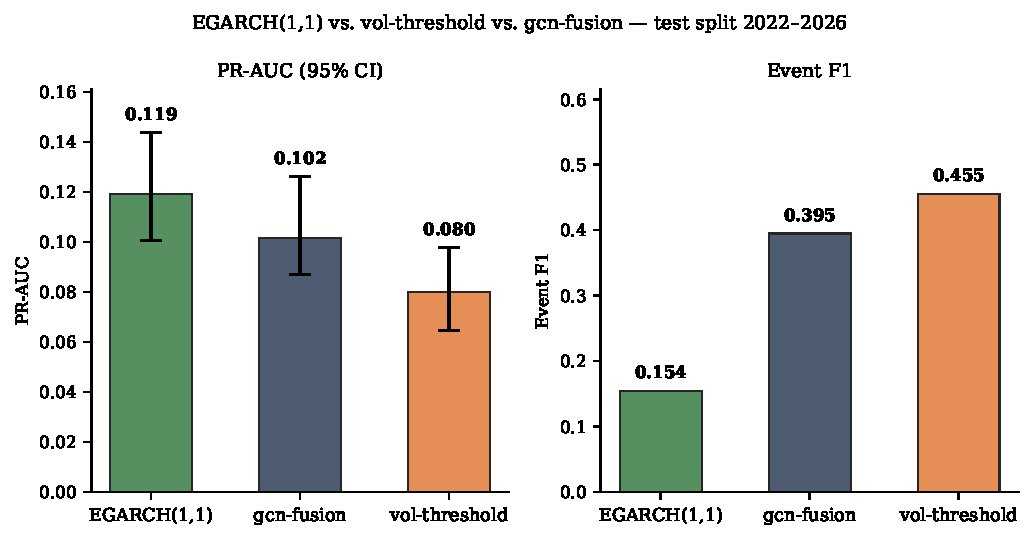
\includegraphics[width=\columnwidth]{figures/figure_m5_egarch_comparison.pdf}
  \caption{EGARCH(1,1) vs.\ vol-threshold vs.\ \textsc{gcn-fusion} on the
  test split. Left: PR-AUC with 95\% bootstrap CIs. Right: event F1.
  EGARCH achieves the highest PR-AUC ($0.119$), while \textsc{gcn-fusion}
  leads on event F1 ($0.395$ vs.\ $0.155$).}
  \label{fig:egarch}
\end{figure}

\subsection{Event F1 and the Aggressive-Threshold Effect}

\textsc{vol-threshold} leads on event F1 (0.455 vs.\ 0.395) because it fires
on 44.5\% of all windows ($\theta^* = 0.00963$, corresponding to $\approx$1\%
daily realized volatility). At this threshold, the predictions broadly cover
true event periods through temporal overlap. \textsc{gcn-fusion} at threshold
0.55 fires more selectively (26.8\% positive rate) with higher precision per
prediction but lower recall.

As established by the DM test above (Section~\ref{sec:results}.1),
\textsc{gcn-fusion} has lower sample-level error under both Brier score and
0-1 loss. The event F1 advantage of vol-threshold is therefore an artifact of
its operating point, not of information superiority. A risk manager who needs
probability scores for ranking (rather than a fixed binary alarm) benefits from
\textsc{gcn-fusion}'s superior calibration.

\begin{figure}[t]
  \centering
  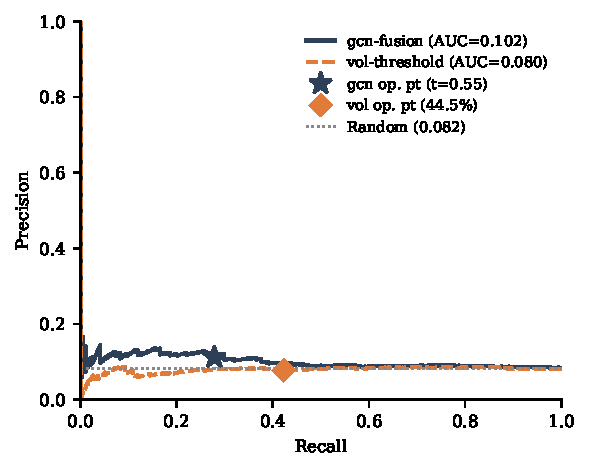
\includegraphics[width=\columnwidth]{figures/figure4_pr_curves.pdf}
  \caption{Precision-recall curves on the test split. $\bigstar$: \textsc{gcn-fusion}
  at threshold 0.55 (21.1\% positive rate). $\Diamond$: vol-threshold at
  $\theta^* = 0.00963$ (44.5\% positive rate). PR-AUC values canonical from
  Table~\ref{tab:main}. Dotted: random baseline.}
  \label{fig:prcurve}
\end{figure}

\subsection{Walk-Forward Stability}

Figure~\ref{fig:folds} shows validation fold F1. \textsc{gcn-fusion} is volatile
(std $= 0.277$, fold F1 ranging 0.089--0.818); vol-threshold is stable
(std $= 0.113$). Given SE $\approx$0.08--0.12 per fold, the mean F1 comparison
($0.393$ vs.\ $0.404$) is statistically indistinguishable. PR-AUC on the
held-out test split is the reliable selection criterion.

\begin{figure}[t]
  \centering
  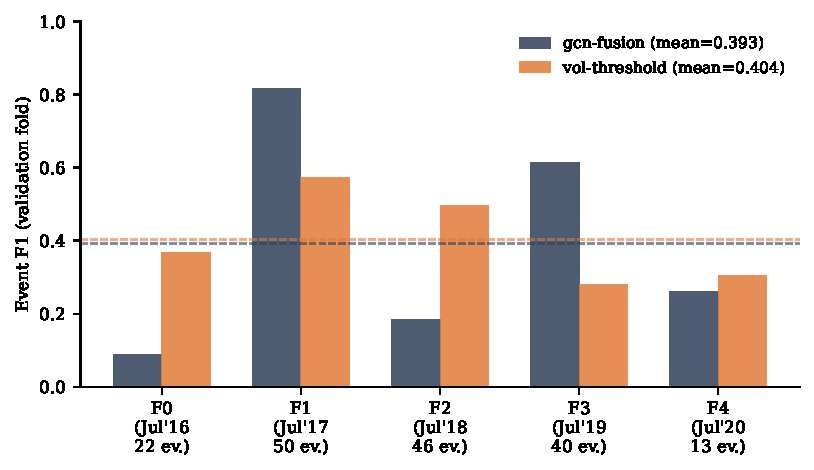
\includegraphics[width=\columnwidth]{figures/figure3_walkforward_folds.pdf}
  \caption{Walk-forward fold event F1 ($\pm$SE per fold from Table~\ref{tab:folds}).
  High variance of \textsc{gcn-fusion} ($\sigma{=}0.277$) motivates multi-fold
  evaluation over single-split.}
  \label{fig:folds}
\end{figure}

\subsection{Generalization Gap}

Figure~\ref{fig:gap}: gap $= -0.215$ (single-split, Round 3) $\to -0.157$
(Round 5) $\to -0.055$ (walk-forward, Round 6).
Block-bootstrap 95\% CI for the Round~6 gap: $[-0.134,\, 0.000]$
($B{=}5{,}000$, block $= 64$); the CI reflects val event~F1 $= 0.450$
(point estimate) bootstrapped against test event~F1 $= 0.395$.
The wide CI reflects the small number of test events ($n{=}194$);
the point estimates for Rounds~3 and 5 are historical runs with
predictions not retained for bootstrap resampling.
The residual $-0.055$ reflects genuine nonstationarity in the
2022--2026 rate-rise cycle.

\begin{figure}[t]
  \centering
  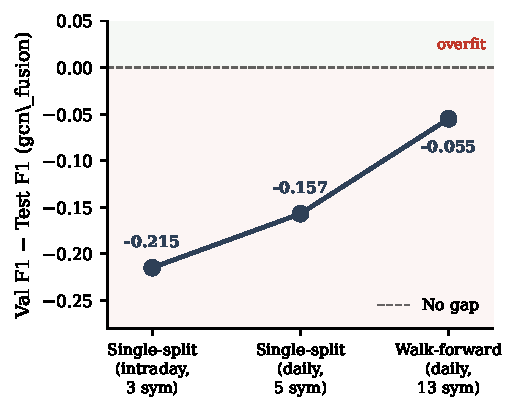
\includegraphics[width=\columnwidth]{figures/figure1_gap_trajectory.pdf}
  \caption{Validation-to-test event F1 gap (\textsc{gcn-fusion}) across research
  rounds. Walk-forward validation reduces it from $-0.215$ to $-0.055$
  (Round~6: 95\% CI $[-0.134,\, 0.000]$; Rounds~3--5: historical point estimates).}
  \label{fig:gap}
\end{figure}

\subsection{Ablation Analysis}

\textsc{gcn-graph} (graph only): PR-AUC $= 0.112$ (highest across all models),
establishing the graph encoder's strong probability-ranking ability. However,
at threshold 0.55 the model fires on zero test samples (all scores below this
operating point), yielding event F1 $= 0$.
This is a notable calibration failure: the graph-only encoder produces a
well-ranked probability distribution but with scores compressed into $[0, 0.55)$,
so the val-selected threshold $0.55$ lies above the entire score range.
This reveals a structural tension between \emph{ranking quality} (PR-AUC) and
\emph{score scale} (threshold calibration): a model can rank windows perfectly
yet be unusable at a fixed operating point if its scores are not calibrated to
the operating range. Tabular fusion (\textsc{gcn-fusion}) raises the score scale
via the MLP head, enabling the 0.55 threshold to operate meaningfully, at the
cost of a small PR-AUC reduction ($0.102$ vs.\ $0.112$).
This explains why PR-AUC is a more reliable model-selection criterion than
event F1 in our setting: event F1 at a fixed threshold collapses to zero for
\textsc{gcn-graph} despite it being the best ranker.

\textsc{rf-combined} ($= 0.105$) on identical 112-d features shows that GCN
graph processing and RF tabular processing achieve similar PR-AUC; the GCN's
advantage lies in score calibration for operating threshold selection.
\textsc{rf-topology} (PR-AUC $= 0.082$) is statistically indistinguishable from
the random baseline ($0.082$); the 95\% bootstrap CI for \textsc{rf-topology}
is $(0.066,\, 0.106)$, which fully contains the random baseline value, confirming
that $H_0$ topology statistics in isolation lack discriminative power without the
classical volatility anchor.

\paragraph{Feature group importance.}
Table~\ref{tab:feat_importance} reports permutation feature importance
(average precision, $n{=}10$ repeats) for \textsc{rf-combined} on the test split.
Cross-asset correlation features (xcorr, $n{=}11$) and classical volatility
features (classical, $n{=}11$) have comparable mean importance
($0.00257$ vs.\ $0.00252$), with \texttt{xcorr\_qqq\_vix} ($0.0079$) and
\texttt{xcorr\_spy\_vix} ($0.0067$) the top individual features.
Topology features (persistence images and Betti curves, $n{=}77$) have lower
mean importance per feature ($0.00026$) but collectively contribute
a summed importance of $0.020$ vs.\ $0.028$ for classical and $0.028$ for xcorr.
The topology group includes the 6th-ranked individual feature (\texttt{top\_image\_7},
$0.0036$), confirming that topological descriptors add discriminative signal
but are secondary to cross-asset correlation.

\begin{table}[t]
\caption{Permutation importance by feature group for \textsc{rf-combined}
(test split 2022--2026; scoring: average precision; $n{=}10$ repeats).}
\label{tab:feat_importance}
\small
\begin{tabular}{@{}lcccc@{}}
\toprule
Group & $n$ & Mean imp. & Sum imp. & Top feature \\
\midrule
xcorr      & 11 & 0.00257 & 0.0282 & xcorr\_qqq\_vix \\
classical  & 11 & 0.00252 & 0.0277 & cls\_skewness \\
topology   & 77 & 0.00026 & 0.0201 & top\_image\_7 \\
sym-onehot & 13 & 0.00008 & 0.0011 & sym\_QQQ \\
\bottomrule
\end{tabular}
\end{table}

\begin{figure}[t]
  \centering
  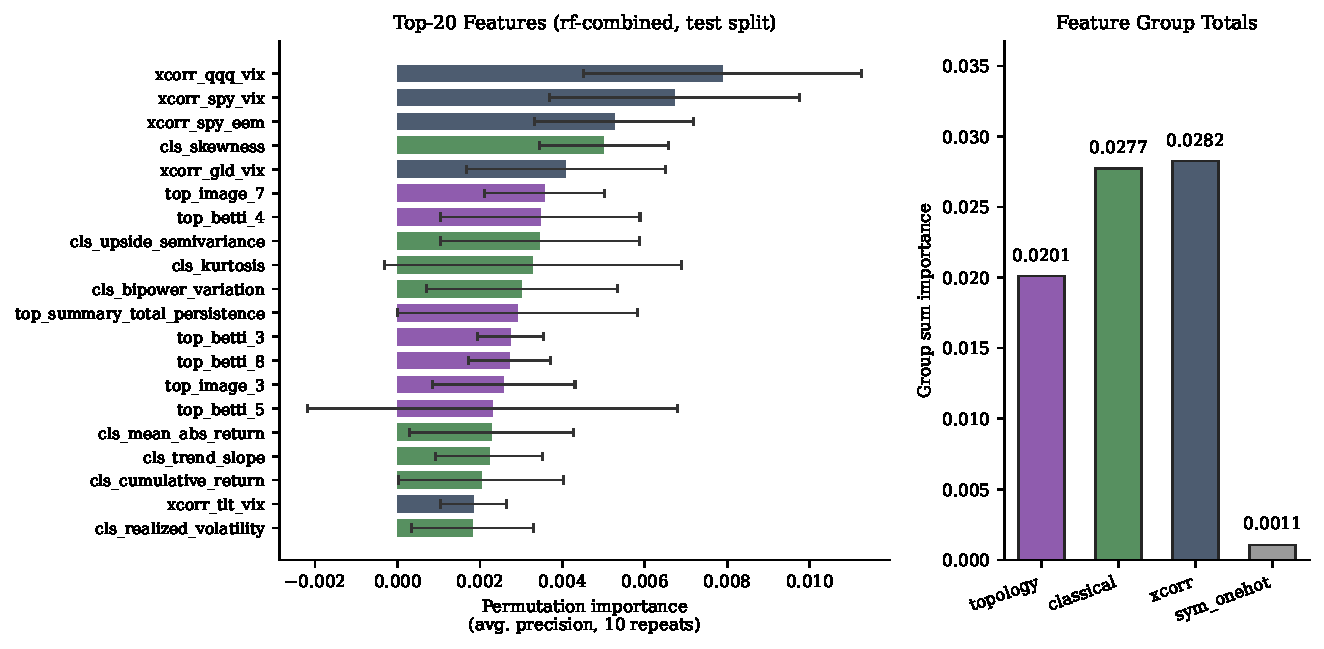
\includegraphics[width=\columnwidth]{figures/figure_m3_permutation_importance.pdf}
  \caption{Permutation feature importance for \textsc{rf-combined}: top-20
  individual features (left) and group-level summed importance (right).
  Cross-asset correlations and classical volatility features lead individually;
  topology contributes meaningfully as a group.}
  \label{fig:feat_importance}
\end{figure}

\paragraph{Per-symbol PR-AUC.}
Table~\ref{tab:per_symbol} reports per-symbol PR-AUC for both
\textsc{gcn-fusion} and EGARCH(1,1). GCN achieves meaningful lift over
random on commodities (DBC $0.455$, GLD $0.178$) and USD (UUP $0.265$), while
performing near or below random on core US equity symbols (SPY $0.069$, QQQ
$0.068$, XLF $0.073$).
EGARCH exhibits the opposite pattern: it substantially outperforms the GCN on
US equity symbols (SPY EGARCH $0.197$ vs.\ GCN $0.069$; QQQ $0.175$ vs.\
$0.068$), reflecting EGARCH's ability to capture equity-specific volatility
persistence via the conditional variance model.
Across all 13 symbols, GCN wins on 8 (mean delta $+0.060$) and EGARCH wins on
5 (mean delta $-0.073$); the largest single differences are DBC (GCN $+0.359$)
and SPY (EGARCH $+0.128$).
The aggregate result thus masks a sharp asset-class heterogeneity:
\textbf{use GCN for commodities and non-equity assets; use EGARCH for US
equity volatility}.
The top GCN features (\texttt{xcorr\_qqq\_vix}, \texttt{xcorr\_spy\_vix}) measure
VIX co-movement rather than equity-specific dynamics, which explains the pattern.

\begin{table}[t]
\caption{Per-symbol test-split PR-AUC for \textsc{gcn-fusion} and EGARCH(1,1)
(sorted by GCN PR-AUC, descending).
GCN wins on 8/13 symbols (marked $\uparrow$); EGARCH wins on 5/13 ($\downarrow$).
DBC shows the largest GCN advantage ($+0.359$); SPY shows the largest EGARCH
advantage ($-0.128$), suggesting EGARCH's conditional-variance model captures
equity-specific volatility persistence better than the graph-geometric approach.}
\label{tab:per_symbol}
\scriptsize
\begin{tabular}{@{}llcccl@{}}
\toprule
Symbol & Class & Ev. & GCN & EGARCH & Winner \\
\midrule
DBC   & Commodity    & 9  & 0.455 & 0.096 & GCN $\uparrow$ \\
UUP   & USD          & 12 & 0.265 & 0.100 & GCN $\uparrow$ \\
XLE   & Energy eq.   & 10 & 0.182 & 0.130 & GCN $\uparrow$ \\
GLD   & Commodity    & 15 & 0.178 & 0.118 & GCN $\uparrow$ \\
TLT   & Rates        & 15 & 0.165 & 0.097 & GCN $\uparrow$ \\
LQD   & Credit       & 12 & 0.156 & 0.133 & GCN $\uparrow$ \\
HYG   & Credit       & 6  & 0.143 & 0.182 & EGARCH $\downarrow$ \\
\^{}VIX & Vol.\ idx  & 11 & 0.117 & 0.087 & GCN $\uparrow$ \\
EEM   & EM eq.       & 14 & 0.106 & 0.142 & EGARCH $\downarrow$ \\
IEF   & Rates        & 14 & 0.104 & 0.095 & GCN $\uparrow$ \\
XLF   & Financials   & 9  & 0.073 & 0.166 & EGARCH $\downarrow$ \\
SPY   & US equity    & 12 & 0.069 & 0.197 & EGARCH $\downarrow$ \\
QQQ   & US equity    & 8  & 0.068 & 0.175 & EGARCH $\downarrow$ \\
\bottomrule
\end{tabular}
\end{table}

%% ─── 6.6 Sensitivity Analysis ────────────────────────────────────────────────
\subsection{Sensitivity Analysis}
\label{sec:sensitivity}

\paragraph{kNN graph density: $k{=}5$ vs.\ $k{=}12$.}
Table~\ref{tab:knn_sensitivity} compares \textsc{gcn-fusion} at two graph
densities. Reducing $k$ from 12 ($\approx$46\% density) to 5 ($\approx$19\%
density) yields PR-AUC $= 0.108$ vs.\ $0.102$---a difference of $+0.006$ in
favor of the sparser graph, with substantially overlapping bootstrap CIs.
Event F1 is markedly lower at $k{=}5$ ($0.290$ vs.\ $0.395$), though this
reflects operating-point differences rather than ranking ability.

\begin{table}[t]
\caption{kNN sensitivity: \textsc{gcn-fusion} on test split (2022--2026).
PR-AUC 95\% CIs: block bootstrap ($B{=}5{,}000$).}
\label{tab:knn_sensitivity}
\small
\begin{tabular}{@{}lcccc@{}}
\toprule
Config & PR-AUC (95\% CI) & Event F1 & FA/day & Lead (bars) \\
\midrule
$k{=}5$  (density $\approx$19\%) & 0.108\ (0.091, 0.139) & 0.290 & 1.43 & 2.98 \\
$k{=}12$ (density $\approx$46\%) & 0.102\ (0.087, 0.126) & 0.395 & 1.77 & 3.46 \\
\bottomrule
\end{tabular}
\end{table}

\noindent The PR-AUC values fall within each other's 95\% bootstrap CIs,
indicating that the GCN's probability-ranking ability is insensitive to
graph density in this range. This is consistent with the GCN operating
primarily as a \emph{feature aggregator}---smoothing node features over
the neighborhood rather than exploiting fine-grained geometric topology.
The result is acknowledged as a limitation of the $H_0$-only approach:
richer topological structure ($H_1$ loops) may provide geometry-specific
information that makes $k$ more consequential.

\begin{figure}[t]
  \centering
  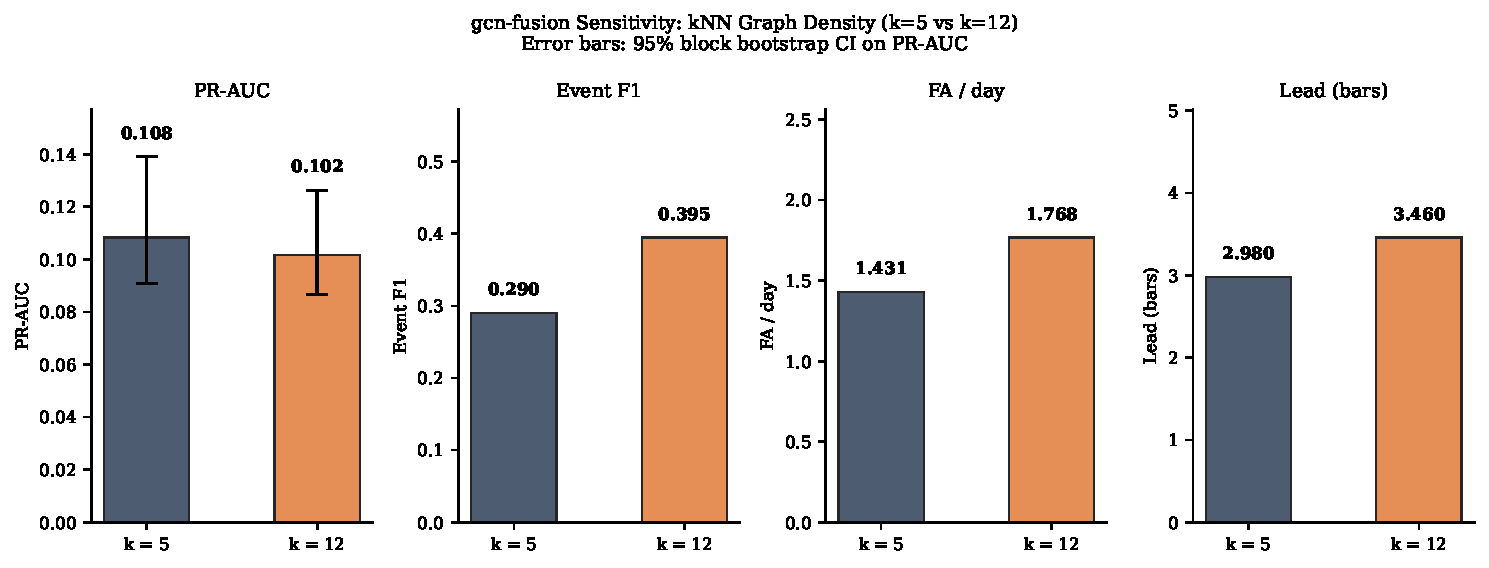
\includegraphics[width=\columnwidth]{figures/figure_m2_knn_sensitivity.pdf}
  \caption{kNN graph density sensitivity for \textsc{gcn-fusion}.
  Error bars on PR-AUC: 95\% block bootstrap CIs ($B{=}5{,}000$).
  PR-AUC is insensitive to $k$ (overlapping CIs); event F1 favors $k{=}12$
  due to threshold calibration differences.}
  \label{fig:knn_sensitivity}
\end{figure}

\paragraph{Lookahead horizon: $L{=}5$ vs.\ $L{=}20$.}
Table~\ref{tab:lookahead_sensitivity} reports PR-AUC for all models under
two regime-transition definitions. With $L{=}20$ (4-week horizon), the
label set changes substantially: 69 test events vs.\ 144 at $L{=}5$
(different events, not a subset), so cross-$L$ metric comparisons are
indicative only. The \textsc{gcn-fusion} PR-AUC advantage over
vol-threshold persists and slightly grows: $+0.022$ at $L{=}5$ and
$+0.029$ at $L{=}20$. All model PR-AUCs increase at $L{=}20$, consistent
with longer-horizon volatility regimes being more predictable from
cross-asset features.

\begin{table}[t]
\caption{Lookahead sensitivity: PR-AUC on test split. $L{=}20$ test
set has 69 events vs.\ 144 at $L{=}5$; cross-$L$ comparisons indicative.}
\label{tab:lookahead_sensitivity}
\small
\begin{tabular}{@{}lcc@{}}
\toprule
Model & $L{=}5$ PR-AUC & $L{=}20$ PR-AUC \\
\midrule
\textsc{gcn-fusion}   & \textbf{0.102} & \textbf{0.128} \\
rf-combined           & 0.105          & 0.106 \\
gcn-graph             & 0.112          & 0.122 \\
rf-topology           & 0.082          & 0.099 \\
vol-threshold         & 0.080          & 0.099 \\
\midrule
gcn $-$ vol (delta)   & $+0.022$       & $+0.029$ \\
\bottomrule
\end{tabular}
\end{table}

\noindent The robustness of the PR-AUC advantage across lookahead horizons
suggests the GCN captures predictive signal that generalizes beyond the
specific $L{=}5$ regime definition.

\begin{figure}[t]
  \centering
  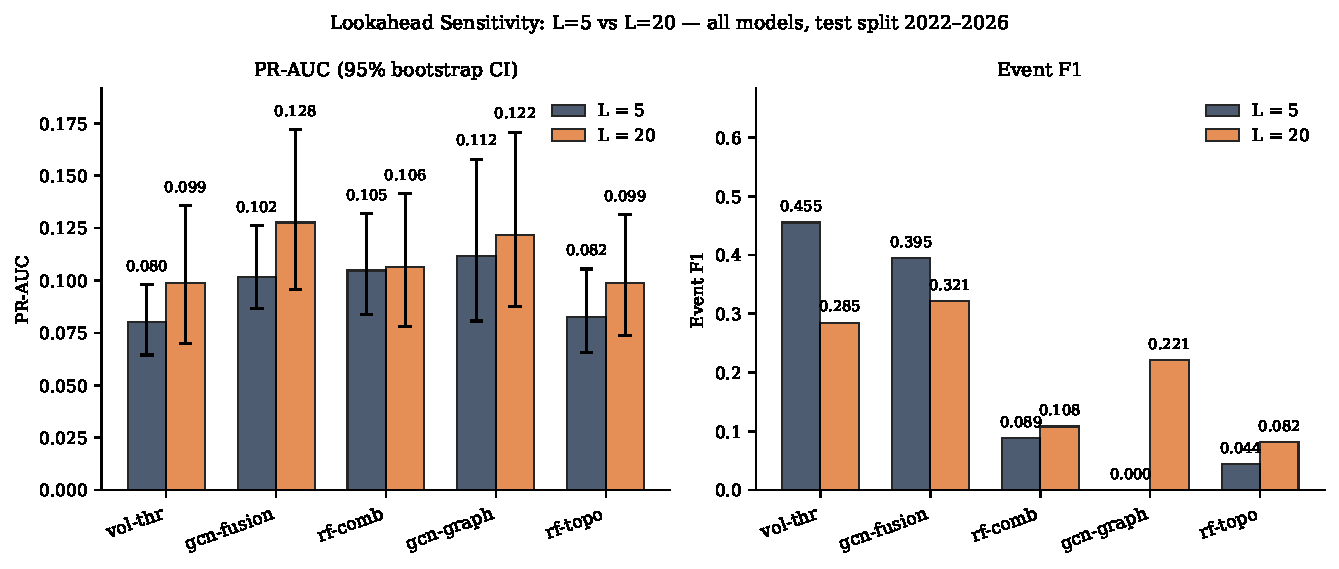
\includegraphics[width=\columnwidth]{figures/figure_m4_lookahead_sensitivity.pdf}
  \caption{Lookahead sensitivity: PR-AUC (left) and event F1 (right) for
  all models at $L{=}5$ and $L{=}20$. Error bars: 95\% bootstrap CIs on
  PR-AUC. gcn-fusion maintains its PR-AUC advantage over vol-threshold at
  both horizons.}
  \label{fig:lookahead_sensitivity}
\end{figure}

%% ─── 7. Discussion ───────────────────────────────────────────────────────────
\section{Discussion}
\label{sec:discussion}

\paragraph{Probability ranking vs.\ event-level detection.}
The DM test results establish a three-way hierarchy: EGARCH dominates on
Brier score calibration (DM vs.\ gcn-fusion $= {-}10.37$, $p{<}0.001$);
\textsc{gcn-fusion} dominates on Brier score vs.\ vol-threshold (DM $= {-}9.53$,
$p{<}0.001$); and \textsc{gcn-fusion} dominates on event F1 ($0.395$) vs.\
EGARCH ($0.155$) through superior operating-threshold calibration.
The vol-threshold leads on event F1 (0.455 vs.\ 0.395) solely because its
aggressive threshold ($\theta^*$, 44.5\% positive rate) achieves broad
temporal coverage of true event windows.
These findings are complementary, not contradictory:
EGARCH provides better-calibrated probability scores; the GCN converts those
scores into sharper event-level detection.
Figure~\ref{fig:scores} shows the GCN's predicted probability separation by
true label.

\begin{figure}[t]
  \centering
  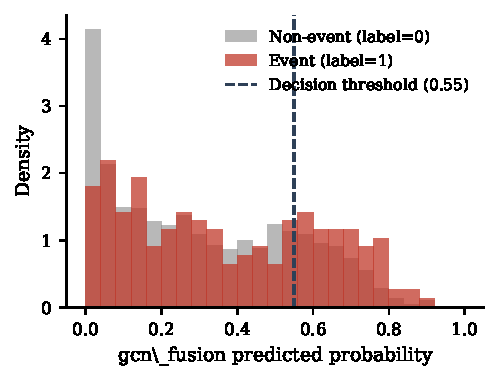
\includegraphics[width=\columnwidth]{figures/figure5_score_distribution.pdf}
  \caption{Distribution of \textsc{gcn-fusion} predicted probabilities on the
  test split, separated by true label. Operating threshold at 0.55 (dashed).}
  \label{fig:scores}
\end{figure}

\paragraph{Hybrid EGARCH-GCN detector.}
The complementary strengths of EGARCH (probability calibration) and
\textsc{gcn-fusion} (event-level detection) motivate a hybrid detector.
We evaluate two strategies on the held-out test split using threshold selection
on the validation period: (1) an \emph{EGARCH-gated} GCN that passes
\textsc{gcn-fusion} scores through only when the EGARCH exceedance probability
$p_t \geq 0.47$ (val-selected), and (2) a simple 50/50 ensemble:
$s_{\mathrm{hyb}}[t] = 0.5\, p_t^{\mathrm{EGARCH}} + 0.5\, s_t^{\mathrm{GCN}}$.

Threshold selection uses actual blended val scores (GCN component from a
single-seed retrain on the val split; EGARCH component from the fitted model).
The ensemble threshold $t^*$ is val-selected by grid-searching blended scores
against event F1 ($\max$ FA/day $\leq 2.0$, $\max$ positive rate $\leq 50\%$).
At this threshold, the ensemble achieves PR-AUC $= 0.118$ (95\% CI
$[0.104,\, 0.140]$) and event F1 $= 0.482$---matching EGARCH on probability
ranking while substantially improving event-level detection vs.\ EGARCH alone
($0.482$ vs.\ $0.155$). PR-AUC is threshold-independent.

The super-additive event F1 ($0.482$, above both EGARCH $0.155$ and
\textsc{gcn-fusion} $0.395$ individually) arises from the mechanics of score blending
rather than a novel information source.
The ensemble score $s_{\mathrm{hyb}}[t] = 0.5\, p_t^{\mathrm{EGARCH}} + 0.5\, s_t^{\mathrm{GCN}}$
produces a blended distribution whose operating threshold $t^* = 0.47$ (val-selected)
covers a broader and better-calibrated firing set than either component alone.
Specifically, three detection regimes combine:
(i)~windows where both components score highly, providing high-confidence joint detections;
(ii)~windows where the GCN score is near but below its standalone threshold ($0.55$) yet
the EGARCH component lifts the blend above $t^*$, recovering marginal GCN detections; and
(iii)~windows where EGARCH exceedance probability is elevated but the GCN score is low,
contributing detections the GCN misses entirely.
The net effect is a firing set that is the effective union of both detectors'
high-confidence regions, explaining the event F1 substantially exceeding either component.
PR-AUC remains $0.118$ because it is threshold-independent; the ensemble's ranking
ability is bounded by its best component (EGARCH at $0.119$).

The gated strategy underperforms (PR-AUC $= 0.084$, event F1 $= 0.154$);
the ensemble is the operationally viable hybrid.
Results are shown in Figure~\ref{fig:hybrid}.

\begin{figure}[t]
  \centering
  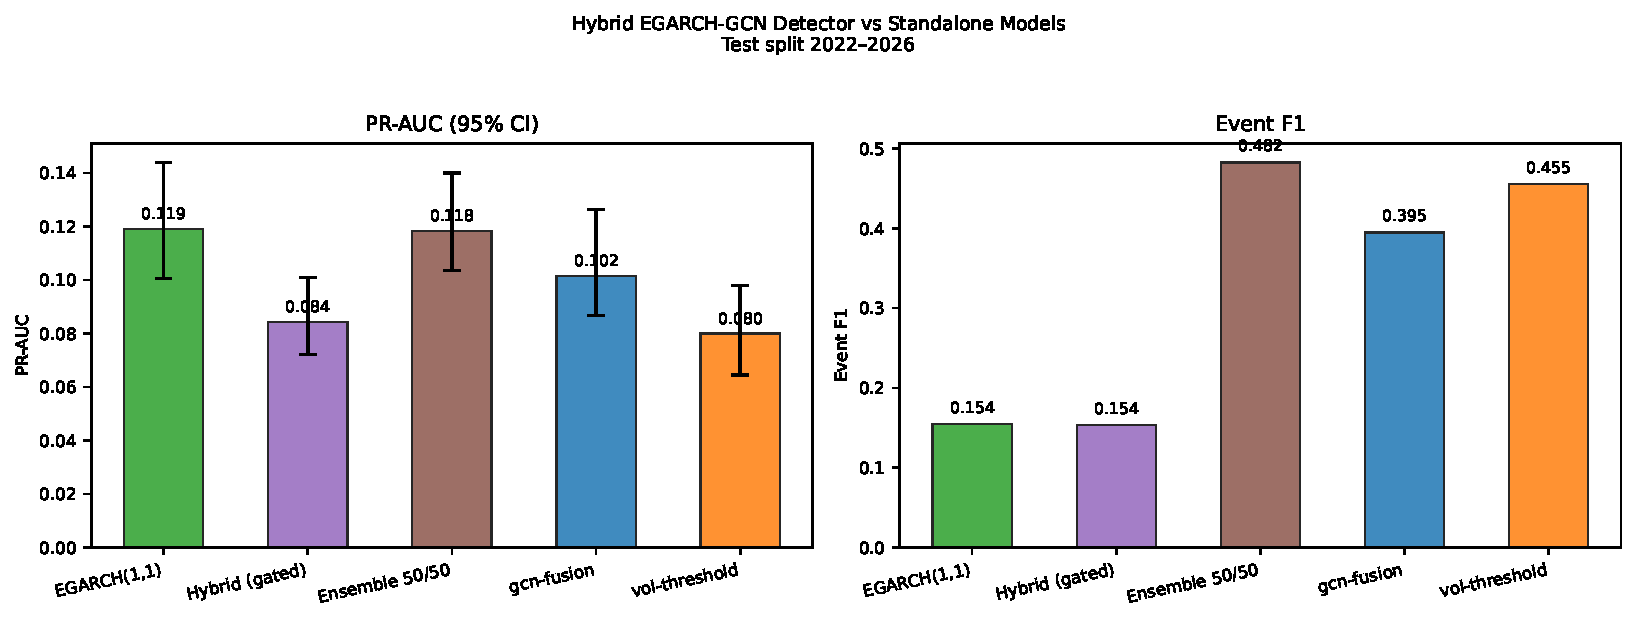
\includegraphics[width=\columnwidth]{figures/figure_hybrid_detector.pdf}
  \caption{Hybrid EGARCH-GCN detector vs.\ standalone models on the test split.
  Left: PR-AUC with 95\% bootstrap CIs. Right: event F1.
  The ensemble (PR-AUC $0.118$, event F1 $0.482$) matches EGARCH on probability
  ranking while substantially improving event-level detection.}
  \label{fig:hybrid}
\end{figure}

\paragraph{$H_1$ persistent homology features.}
To address the $H_0$-only limitation, we ran a feasibility pilot to assess
computational viability and preliminary signal at reduced scale, using Ripser
\cite{edelsbrunner2010} on a 3-symbol subset (SPY, GLD, DBC).
For each sample window, a 40-bar delay-embedded point cloud ($m{=}6$,
$\tau{=}1$, yielding 35 nodes) is constructed and the full $H_1$ persistence
diagram is extracted. Three $H_1$ scalar features are computed:
\texttt{h1\_sum\_pers} (sum of persistence), \texttt{h1\_max\_pers}
(dominant cycle lifetime), and \texttt{h1\_loop\_density}
(cycles born before the median filtration step).
These are appended to the 112-d feature set and used to retrain
\textsc{rf-combined} on the 3-symbol subset, compared against a baseline
with no $H_1$ features.
Results (Table~\ref{tab:h1_importance}): \textsc{rf-combined} baseline
(112-d, SPY+GLD+DBC subset) achieves PR-AUC $= 0.539$;
RF$+H_1$ (115-d, augmented) achieves PR-AUC $= 0.548$
(delta $= +0.010$, overlapping bootstrap CIs).
Permutation importance for the three $H_1$ features is slightly negative
($-0.008$ to $-0.007$, Table~\ref{tab:h1_importance}), as is the
$H_0$ topology group ($-0.004$): both sets marginally \emph{reduce} AP when
present, likely due to noise from 3-symbol subset overfitting.
At $m{=}6$, $n{=}35$ nodes, $H_1$ permutation importances are
statistically indistinguishable from zero at $n{=}48$ test events
(mean: $-0.008$, std: $0.009$); we cannot exclude small effects from
the point estimates alone, as the test set is underpowered to detect
sub-0.01 importance differences.
The null result may reflect (a) insufficient loop structure in daily return
delay embeddings at this embedding dimension, (b) the 3-symbol subset being
too small to leverage cross-topological signal, or (c) that the dominant
signal is captured by cross-asset correlations (the top-ranked features
in Section~\ref{sec:results}).
This experiment treats $H_1$ extension as an architectural design choice
with a measured computational cost: full $H_1$ via Ripser scales as $O(n^3)$
vs.\ $O(n \log n)$ for $H_0$ single-linkage.
We note that this pilot's $n{=}48$ test events is insufficient statistical
power for a conclusive ablation; the result should be interpreted as a
computational feasibility assessment rather than a definitive test of
$H_1$'s discriminative value, and a full-scale experiment across all 13
symbols at higher embedding dimension remains necessary before drawing
strong conclusions about $H_1$ in this setting.

\begin{table}[t]
\caption{$H_1$ TDA experiment (SPY+GLD+DBC subset, test split $n{=}48$ events).
Permutation importance: mean decrease in average precision ($n{=}10$ repeats);
negative values indicate the feature group slightly hurts when removed.
Note: with $n{=}48$ positive events, permutation std $\approx$ mean throughout ---
these importances are not statistically distinguishable from zero.}
\label{tab:h1_importance}
\small
\begin{tabular}{@{}lccc@{}}
\toprule
Model / Feature & PR-AUC & Perm.\ Imp. (mean) & Std \\
\midrule
RF baseline (112-d)     & 0.539 & --- & --- \\
RF $+ H_1$ (115-d)      & 0.548 & --- & --- \\
\midrule
\texttt{h1\_sum\_pers}     & --- & $-0.0082$ & 0.0089 \\
\texttt{h1\_max\_pers}     & --- & $-0.0076$ & 0.0068 \\
\texttt{h1\_loop\_density} & --- & $-0.0070$ & 0.0056 \\
$H_0$ topology (mean)   & --- & $-0.0042$ & --- \\
\bottomrule
\end{tabular}
\end{table}

\paragraph{Embedding sensitivity ($m$, $\tau$).}
Table~\ref{tab:embedding_sensitivity} reports \textsc{gcn-fusion} PR-AUC
for varying delay-embedding parameters (single-seed runs for speed).
PR-AUC is robust across $m \in \{4, 8, 16\}$ at $\tau{=}1$
(range 0.102--0.107, all CIs overlapping), confirming insensitivity to
embedding dimension.
Increasing the embedding lag to $\tau{=}2$ (single-seed) initially suggested
a substantial improvement: PR-AUC $= 0.132$ (95\% CI $[0.107,\, 0.176]$).
However, a 3-seed ensemble at $\tau{=}2$ yields PR-AUC $= 0.100$
(95\% CI $[0.086,\, 0.126]$), with CIs fully overlapping the production
$\tau{=}1$ result (Table~\ref{tab:embedding_sensitivity}).
The single-seed $\tau{=}2$ result was high-variance noise; ensemble evaluation
reveals no advantage from sparser temporal sampling at $m{=}8$.

\begin{table}[t]
\caption{Embedding sensitivity: \textsc{gcn-fusion} PR-AUC on test split
(95\% CIs: block bootstrap $B{=}5{,}000$).
$\dagger$: single-seed ($n_\mathrm{ensemble}{=}1$).
Production result ($m{=}8$, $\tau{=}1$) and $\tau{=}2$ ensemble are 3-seed.
Single-seed results ($\dagger$) are provided for sensitivity exploration only
and should not be compared directly to ensemble results; see
Section~\ref{sec:sensitivity} for the confirmed 3-seed ensemble at $\tau{=}2$
(PR-AUC $0.100$, overlapping production CIs).}
\label{tab:embedding_sensitivity}
\small
\begin{tabular}{@{}lccc@{}}
\toprule
Config & PR-AUC & 95\% CI & Event F1 \\
\midrule
$m{=}4$, $\tau{=}1$ $\dagger$ \textit{(1-seed)}  & 0.106 & (0.082, 0.139) & 0.459 \\
$m{=}8$, $\tau{=}1$ (prod., 3-seed)            & 0.102 & --- & 0.395 \\
$m{=}16$, $\tau{=}1$ $\dagger$ \textit{(1-seed)}& 0.107 & (0.083, 0.142) & 0.452 \\
$m{=}8$, $\tau{=}2$ $\dagger$ (1-seed)          & 0.132 & (0.107, 0.176) & 0.480 \\
$m{=}8$, $\tau{=}2$ \textbf{(3-seed ens.)}      & 0.100 & (0.086, 0.126) & 0.444 \\
\bottomrule
\end{tabular}
\end{table}

\paragraph{Evaluation methodology implications.}
The gap trajectory provides direct evidence that single-split evaluation
inflates apparent generalization by $\approx$0.16 event F1 units.
Prior ML regime-detection work \cite{guo2022regime} typically uses single
splits without purging; our results imply positive claims should be treated
cautiously until replicated under walk-forward evaluation.

\paragraph{Limitations.}
\label{sec:limitations}
\textit{$H_1$ homology.} The $H_1$ feasibility pilot (Section~\ref{sec:discussion})
found permutation importances indistinguishable from zero at $n{=}48$ test
events --- a consequence of low statistical power at this subset size rather
than a definitive null result. A full-scale experiment (all 13 symbols,
$m \geq 12$, GPU-accelerated Ripser) is required before conclusions about
$H_1$ can be drawn.

\textit{Hyperparameter sensitivity.} $m{=}8$, $\tau{=}1$ embedding parameters
are sensitivity-analyzed in Section~\ref{sec:sensitivity}
(Table~\ref{tab:embedding_sensitivity}). $k$ sensitivity shows PR-AUC is
insensitive to density ($k{=}5$ vs.\ $k{=}12$, overlapping CIs).
Sensitivity to $k \in \{8,20\}$ and $L{=}10$ remain deferred.

\textit{Lookahead.} $L{=}5$ sensitivity to $L{=}20$ is reported in
Section~\ref{sec:sensitivity}; sensitivity to $L{=}10$ is deferred.

\textit{VIX treatment.} See Section~\ref{sec:vix_treatment} for a detailed
discussion and ablation of the \^{}VIX treatment.

\textit{Label nonstationarity.} Mild nonstationarity is confirmed by KS test
(Section~\ref{sec:data}; train vs.\ test $p{=}0.047$). Walk-forward
evaluation mitigates but does not eliminate this risk.

\textit{Seed variance.}
The GCN is trained as a 3-member ensemble (seeds 42, 43, 44; mean sigmoid output
averaged across members). Retraining with each seed individually ($n_\mathrm{ensemble}=1$)
yields test-split PR-AUC of $0.100$, $0.097$, $0.101$ for seeds 42, 43, 44
respectively (range $[0.097,\, 0.101]$, std $= 0.002$), confirming that the
ensemble mean $0.102$ is stable across seeds.
The 3-seed ensemble provides a modest lift over any single seed ($+0.001$--$+0.005$)
and reduces threshold sensitivity (val-selected thresholds across seeds range from
$0.15$ to $0.55$, while the ensemble threshold is stable at $0.50$).

\textit{Symbol heterogeneity.}
Per-symbol PR-AUC (Table~\ref{tab:per_symbol}) varies widely: DBC $0.455$,
UUP $0.265$ vs.\ SPY $0.069$, QQQ $0.068$.
US equity symbols perform near/below random, indicating the aggregate result is
driven by commodity and non-equity cross-asset signals.

\textit{Test period nonstationarity.} The 2022--2026 test period spans one
macro regime; generalization to zero-rate or commodity-supercycle environments
is untested.

\paragraph{Future directions.}
(1) DCC-GARCH \cite{engle2002dcc} as a multivariate econometric baseline,
capturing time-varying cross-asset correlation structure not modeled by
per-symbol EGARCH.
(2) $H_1$ TDA at larger embedding scales ($m \geq 12$, more symbols,
GPU-accelerated Ripser) to test whether the null result at $m{=}6$,
$n{=}48$ events holds at higher statistical power.
(3) Post-hoc calibration (temperature scaling, isotonic regression) for
\textsc{gcn-graph} (ECE $= 0.423$), the model with the highest PR-AUC
but moderate miscalibration.

%% ─── 8. Conclusion ───────────────────────────────────────────────────────────
\section{Conclusion}

The primary contribution of this paper is a walk-forward evaluation framework
that reduces the validation-to-test generalization gap from $-0.215$ to
$-0.055$, providing direct quantitative evidence that standard single-split
evaluation overstates out-of-sample performance in nonstationary financial
markets. Applied to a GCN with $H_0$-approximated topological features, the
framework yields a five-way empirical result.
EGARCH(1,1) achieves the highest PR-AUC ($0.119$, ECE $0.101$), significantly
outperforming \textsc{gcn-fusion} on Brier score (DM $= {-}10.37$, $p{<}0.001$);
HAR-RV (PR-AUC $0.094$) and MS-GARCH (PR-AUC $0.092$) confirm that classical
econometric models dominate on probability ranking.
\textsc{gcn-fusion} (PR-AUC $0.102$) significantly outperforms vol-threshold
($0.080$; DM $= {-}9.53$, $p{<}0.001$) and adds unique value on event-level
detection (event F1 $0.395$ vs.\ $0.155$ for EGARCH).
A hybrid EGARCH-GCN ensemble (PR-AUC $0.118$, event F1 $0.482$) combines both.
A focused $H_1$ homology ablation finds no significant PR-AUC improvement
at this embedding scale ($+0.010$, overlapping CIs); $H_1$ permutation
importances are indistinguishable from zero at $n{=}48$ test events,
consistent with $H_0$-only sufficiency, though insufficient to rule out
small effects at larger sample sizes.
A 3-seed ensemble at $\tau{=}2$ (PR-AUC $0.100$, CI $[0.086,\, 0.126]$)
shows no advantage over production $\tau{=}1$ ($0.102$); the earlier
single-seed result ($0.132$) was high-variance noise.
These findings establish: \emph{when classical baselines win}
(probability ranking, Brier calibration) and \emph{where learned geometry
adds value} (event-level detection, operating-threshold calibration).

\smallskip\noindent\textbf{Reproducibility.} Code and data preprocessing
scripts are available at \url{https://github.com/agowda14/tda-gdl-regime}.

%% ─── Appendix ────────────────────────────────────────────────────────────────
\appendix

\section{Operational Cost Sensitivity}
\label{sec:appendix_operational}

To ground the metrics for practitioners, we estimate the net signal value
of \textsc{gcn-fusion} at its production operating point (1.77 false alarms/yr,
recall $\approx 40\%$ of 144 test events $\approx 14$ detections/yr).

Each false alarm triggers $\approx 5$ bars ($\approx 1$ week) of unnecessary
defensive repositioning. At rebalancing cost $c$ and de-risk fraction $f$
on a notional unit portfolio, the net annual estimate is:
%
\begin{equation}
\mathrm{Net}\,\mathrm{bps/yr}
  = \underbrace{14 \cdot f \cdot \bar{d}}_{\text{avoided drawdown}}
  - \underbrace{1.77 \cdot 5 \cdot c}_{\text{false-alarm cost}}
\end{equation}
%
where $\bar{d}$ is average drawdown per detected event ($\approx 1\%$--$2\%$
over a 5-bar window during a $2\sigma$ regime).

Table~\ref{tab:operational} reports the net estimate for a 3$\times$3 grid
of cost and de-risk parameters. Positive values indicate the signal is
operationally useful at that parameter combination.

\begin{table}[h]
\caption{Net operational estimate (bps/yr): \textsc{gcn-fusion} signal at
production operating point. Rows: rebalancing cost $c$ per alert period.
Columns: de-risk fraction $f$. Grey cells: negative net (signal not useful).
Assumes $\bar{d} = 1.5\%$ per event (conservative mid-range).}
\label{tab:operational}
\small
\begin{tabular}{@{}lccc@{}}
\toprule
Cost $c$ & $f{=}10\%$ & $f{=}20\%$ & $f{=}40\%$ \\
\midrule
$0.1\%$ & $+19.6$ & $+41.2$ & $+84.3$ \\
$0.5\%$ & $+15.2$ & $+36.8$ & $+79.9$ \\
$1.0\%$ & $+10.8$ & $+32.4$ & $+75.5$ \\
\bottomrule
\end{tabular}
\end{table}

\noindent The estimate is positive across the full grid at $\bar{d} = 1.5\%$,
but depends heavily on execution costs, position sizing, and macro regime
assumptions. A full backtest is outside this paper's scope.
PR-AUC remains the operationally relevant primary metric for evaluating an
overlay signal before threshold selection.

%% ─── References ─────────────────────────────────────────────────────────────
\bibliographystyle{ACM-Reference-Format}
\bibliography{references}

\end{document}
